
\section{Simulate}\seclab{Sim}

The purpose of \verb!"Simulate.sh"! or  \verb!"Simulate.bat"! is to simulate various source structures and text how these pass through the imager and has been used in~\cite{Scholten:2022}.

The file names to be processed are read from  \verb#`Simulate.in'# and \verb#`SimIntf.in'#  looking like

\begin{linenumbers}
%\tiny
\resetlinenumber
\begin{verbatim}
&Parameters
 Antennas="simulation/S1-1",
 Simulation="simulation/Discr"
 SrcNrMax = 1000
 NtSamples=1000
 TimingErr_ns = 1.
! FracGalacNoisePow=0.5
 OutFileLabel="tst"  , &end
  0.0  20.35,   18.65,    4.15,      -200.0 200. 300.       !  "Slant_500"
 Cloud 40. 10. 0.1 1000              ! 100% error                         !  cloud
  300.0  20.35,   18.65,    4.15,      -20.0 20. 30.       !  "Slant_50"
 Repeat 150 4         !  "ASync"
  0.0  20.35,   18.64,    4.15,      -300.0 300. 450.       !
\end{verbatim}
\end{linenumbers}

\begin{enumerate*}
\item[2] \verb#' Antennas="simulation/S1-1",'#: The information on the positions of the antennas is read from these files in the "files" subfolder. These files are most efficiently created with the `SelectData' option as discussed in \secref{SelDat}. Note that exclusively the antenna positions are used.
\item[3] \verb#' Simulation="simulation/Discr" '#:  The place in the "files" folder where the simulation results are written.
\item[4] \verb#' SrcNrMax = 1000'#:  The maximum number of single point sources that can be simulated.
\item[4] \verb#' NtSamples=1000'#:  The maximum length (in samples) of the time trace. The minimal number is 400 samples and will be rounded up to a power of 2.
\item[5] \verb#' TimingErr_ns = 1.'#:  The standard deviation of the calibration-timing-error that are assigned to each antenna.
\item[6] \verb#'! FracGalacNoisePow=0.5'#: relative fraction of galactic noise to the total noise. Galactic noise has a 1/frequency spectrum, while instrumental noise is taken to be flat. In actual calculations this hardly matters.
\item[7] \verb#' OutFileLabel="tst",'#:  Additional label for results files.
\item[8] \verb#'   0.0  20.35,   18.65,    4.15,      -200.0 200. 300.   '#:  A point source is put at time=0 [samples] and position (N,E,h)=(20.35, 18.65, 4.15)~km with dipole strength in direction (N,E,h)=(-200.0 200. 300.). A dipole strength of 1. will show with the same amplitude as the noise when the source is placed at a favorable angle at a distance of 1~km from the antenna. There may be many lines like this one. Note that the times of the produced traces is shifted such as to put the first source at sample 200 for the reference antenna.
\item[9] \verb#' Cloud 40. 10. 0.1 1000  '#: Put a cloud of 1000 single point-sources as specified in the following line with a standard deviation of spread in time of 40~[samples], in 3D-position of 10~[m], and in 3D-polarization of 0.1
\item[11] \verb#' Repeat 150 4'#:  Place 4 sources with the same properties at the same position at time intervals of 150 samples.
\end{enumerate*}

\subsection{Output files and print-out}%\seclab{RFI-out}

The generated output files have a very similar structure as those discussed in \secref{SelDat-out}.
The files will be used as input when running the impulsive of the TRI-D imager with option \verb!`Simulation="simulation/Discr" '!
The traces are constructed starting 200 samples before the time of the first source (at the correct time calculated from the position of the first source and the position of the antenna).
Thus, is the first source is at sample 0, the interferometry could be run with  $t=-0.011$ and sample offset 2000 to have the beginning of the investigated trace at the beginning of the generated background. Note that the first source may be 'fake' and have zero intensity.

\subsection{Power calibration}\seclab{PowerCal}

\subsubsection{Pulse}
Starting definitions:
\\$M_{e/o}^a[t] = $ time trace as results from reading the data in ant-read.f90, i.e. filtered and normalized, for one antenna labeled by $a$. $N_{e/o}$ are the corresponding averaged norm factors for even and odd antennas with on average $N_{e/o}=1/{\rm NormEvenOdd}$ with ${\rm NormEvenOdd}=100.$ and are canceled in reading data.
\\$D^a_p[t] =$ time trace used in the TRI-D fitting of the dipole moments. Here $a$ is the label of an antenna pair and $p$ stands for azimuth or zenithal polarization of the field seen by the antenna.
\\${\cal F}$ labels the fourier transform from time to frequency, $J[\theta,\phi](\nu)$ the antenna function transforming from $\nu_p$ (polarization direction) to $\nu_{e/o}$ antenna direction.
\\$G_0[\nu] =\sqrt{(\sum_p\sum_{e/o} J^2[0,0](\nu))/\Delta_\nu}$ is the antenna gain for the vertical direction, where $\Delta_\nu$ is the total bandwidth, typically 30--80~MHz.
Now
\beq
D^a_p[t] =  {\cal F}^{-1}\left(  G_0[\nu]\, J^{-1}\left( N_{e/o}\,{\cal F}(M_{e/o}[t]) \right) \right) \;,
\eeq
omitting the obvious antenna label and noting that this may be complex. This is fitted by the TRI-D fitter (per time sample) to
\beq
{\rm TRI}^a_p[t]=  \vec{p} \cdot \vec{I}[t] /R \;,
\eeq
where $R$ is the antenna-source distance.  $\vec{I}[t]$ is used for calculating the stokes parameters from $Stokes=(1/N_t)\sum_t \vec{I}^\dagger \vec{I}$ where $N_t$ is the number of time samples.

In the simulations we define in addition:
\\$\delta[\nu] = {\cal F} \delta[t]$ where $\delta[t]$ is a time trace equal to zero except for one sample where it equals unity.
\\${\cal I}[t] = {\cal F}^{-1} G_0[\nu] \, \delta[\nu]$ is the impulse response for a source that is vertically overhead to an antenna.
\\$\vec{I}_s = $ source dipole vector. $N_I=$ norm factor relatively arbitrarily set to $N_I=20 \sqrt{14} /TotalGain$
The simulated time trace, $S^a_{e/o}[t]$, that is written to file, is
\beq
S^a_{e/o}[t] = \frac{1}{N_{e/o}} \,N_I\, \Re {\cal F}^{-1}\left( J[\theta,\phi] \left( \vec{p} \cdot \vec{I}_s \right) \delta[\nu] /R \right)
\eeq
where the viewing angles to the source, $[\theta,\phi]$, depend on antenna number $a$ and where on reading-in this trace using the simulation option $N_{e/o}=1/{\rm NormEvenOdd}$ is set, equal to the average when reading real data.

When pulling the simulated data through the TRI-D procedure for the data we obtain
\beq
D^S_p[t] = N_I\,{\cal F}^{-1}\left(  G_0[\nu]\times \left( \vec{p} \cdot \vec{I}_s \right) \delta[\nu] /R \right) \;,
\eeq
using $G_0[\nu] J^{-1}\,J =G_0[\nu] \delta_{p,p'}$ where the factor $G_0$ prevents dividing by zero, and ${\cal F}^{-1} {\cal F}=1$.
To numerically agree with the result from the TRI-D imager we thus obtain
\beq
\vec{I}[t] = N_I\,{\cal F}^{-1}\left(  G_0[\nu]\times \delta[\nu]  \right)\, \vec{I}_s \;.
\eeq
Since $St_I=(1/N_t)\,\sum_t |\vec{I}[t]|^2$ we obtain by putting $|\vec{I}_s |^2=St_I$
\beq
St_I = |\vec{I}_s|^2 \frac{N_I^2}{N_t} \sum_t \left| {\cal F}^{-1}\left(  G_0[\nu]\times \delta[\nu]  \right) \right|^2 \;,
\eeq
as the conversion factor between the input values for the dipole moments in the simulation program to the [gb] units used in TRI-D.

The background power level in the simulation program is set to the same value as used in the LOFLI code.

The results for a source in the simulation code are:
\begin{verbatim}
TRI-D re-norm 0.0214, Intensity at window edge= 0.0018% of peak, TotalGain=   17.869, slicing window IntfSmoothWin= 50
   #  Dt[smpl]   t[smpl]     (N,E,h) [km]                   Ampl(N,E,h)               I123_TRI-D
   1     0.00      0.0     -0.4160    0.5590   45.0000     -0.10    0.00    0.00          0.00
   2  1010.06   1010.0     -0.4260    0.5590   45.0000   2000.10    0.00    0.00       1824.43
   gives
Station=  1        3 CS003 uses 4 antenna pairs. Start time=   0.14916[ms]
 * background power/sample=  0.99984436946070021        1.0122509563864033
 * total power in background=   4095.3625373110281        4146.1799173587078
 * power in sources only:   27196.887091213786        26836.486063132907
 * total power, backgr + sources=   31292.249628524776        30982.665980491667
 Ave background power (all antennas)=  1.   1.006  N_even=N_odd= 162  Tracelength= 4096 samples
\end{verbatim}
\Omit{  -------------------- Omitted
from which we deduce that a source of $1824.43$~[gb] over a slice of $\Delta t=250$~ns (50 samples), straight overhead and transversely polarized, deposits an total energy of $27,016/4,096=6.6$ times that deposited by noise as seen by LOFAR after amplifiers over a time span of $4,096\times 5=20.48$~$\mu$s.
The noise of the LOFAR antenna corresponds to $P_{gb,K}=1.3\times 10^{-14}$~W/MHz Galactic background and the total background measured (if due only to gb) would correspond to a flux of $P_{n,K}=2.2\times 10^{-14}$~W/MHz (see discussion in \secref{SimBckgr}).
The total energy deposited thus corresponds to $E_a(D)=6.6\times 2.2\times 10^{-14} \times 20.48\times 10^{-6}=3\times 10^{-18}$~J/MHz (note different units).
A source emitting a short pulse with a power of $E_s$~[J/MHz] (transverse) vertically above an antenna $a$ at a distance of 45km ($D^2=2.03\times 10^3$~km$^2$) will deposit a pulse with energy $E_a$ obeying
\beq
E_s=0.5\times 4\pi \frac{D^2}{A_a} \times E_a \;J/MHz
\eeq
where the first factor $0.5\times 4\pi$ is due to the integration of the dipole intensity over solid angle and the effective area of the antenna is taken equal to $A_a=\lambda^2/4=25/4=6.25$~m$^2$.
Putting factors together we get that a source with strength $St_I$~[gb] thus emits a total energy of
\bea
E_s &=& 2\pi \frac{D^2}{A_a} \times \frac{St_I\times \Delta t}{1824.43\,[gb]\times 250\,[ns]} \left(\frac{45\,[km]}{D}\right)^2 \times 3\times 10^{-18}\,[J/MHz] \nonumber \\
&=&  2\pi \frac{45^2\,[km]^2}{A_a} \frac{1}{1824.43\times 2.50} \times 3\times 10^{-18} \times \frac{St_I\times \Delta t}{1\,[gb]\times 100\,[ns]}\, [J/MHz] \nonumber \\
&=&  2\pi \times 2.03 \times 10^9 \frac{1}{1824.43\times 2.50} \frac{1\,m^2}{A_a}\times 3\times 10^{-18} \times \frac{St_I\times \Delta t}{1\,[gb]\times 100\,[ns]}\, [J/MHz]  \nonumber \\
&=& \frac{1\,m^2}{A_a} 8.4 \times 10^{-12} \times \frac{St_I\times \Delta t}{1\,[gb]\times 100\,[ns]}\, [J/MHz]
\eea
putting the antenna effective area of $A_a(60MHz,\theta=0,\phi=0)=1$~m$^2$ as used by Katie in making her Figure 5 where the true area is included in the gain factor.

\subsubsection{revised}\seclab{rev-pulse}
} % --------------------end Omit

from which we deduce that a source of $1824.43$~[gb] over a slice of $\Delta t=250$~ns (50 samples), straight overhead and transversely polarized, deposits an total energy of $27,016/4,096=6.6$ times that deposited by noise as seen by LOFAR, after amplifiers, over a time span of $4,096\times 5\times 10^{-9}=20.48 \times 10^{-6}$~s.

The noise of the LOFAR antenna corresponds to $P_{gb,K}=1.3\times 10^{-14}$~W/MHz Galactic background and the total background measured (if due only to gb) would correspond to a flux of $P_{n,K}=2.2\times 10^{-14}$~W/MHz (see discussion in \secref{SimBckgr}).
The total energy deposited thus corresponds to $E_a(D)=6.6\times 2.2\times 10^{-14} \times 20.48\times 10^{-6}=3\times 10^{-18}$~J/MHz (note units).

A source emitting a short pulse with a power of $E_s$~[J/MHz] (transverse) vertically above an antenna $a$ at a distance of 45km ($D^2=2.03\times 10^3$~km$^2$) will deposit a pulse with energy $E_a$ obeying
\beq
E_s=8\pi/3 \frac{D^2}{A_a} \times E_a \;J/MHz
\eeq
where the first factor $8\pi/3$ is due to the integration of the dipole intensity over solid angle ( the electric field is proportional to sinus and the power the square of the E field, giving $$\int \sin^2(\theta) d[\cos(\theta)] d\phi=2\pi \int_{-1}^{+1} (1-x^2)\,dx=4\pi(1-1/3)=8\pi/3$$). The effective area of the antenna is often taken equal to $A_a=\lambda^2/4=25/4=6.25$~m$^2$, however, Katie used in making her Figure 5, an antenna effective area of $A_a(60MHz,\theta=0,\phi=0)=1$~m$^2$ where the true area is included in the gain factor.
Putting factors together we get that a source with strength $St_I$~[gb] thus emits a total energy of
\bea
E_s &=& 8\pi/3 \frac{D^2}{A_a} \times \frac{St_I\times \Delta t}{1824.43\,[gb]\times 250\,[ns]} \left(\frac{45\,[km]}{D}\right)^2 \times 3\times 10^{-18}\,[J/MHz] \nonumber \\
&=& 8\pi \frac{45^2\,[km]^2}{A_a} \frac{1}{1824.43\times 2.50} \times 10^{-18} \times \frac{St_I\times \Delta t}{1\,[gb]\times 100\,[ns]}\, [J/MHz] \nonumber \\
&=& 8\pi \times 2.03 \times 10^9 \frac{1}{1824.43\times 2.50} \times 10^{-18} \times \frac{St_I\times \Delta t}{1\,[gb]\times 100\,[ns]}\, [J/MHz]  \nonumber \\
&=&  1.1 \times 10^{-11} \times \frac{St_I}{[gb]} \times \frac{\Delta t}{100\,[ns]}\, [J/MHz]
\eea

\Omit{
\subsubsection{Background-Old}\seclab{SimBckgr-Old}
The brightness temperature of radiation is given by $T_b = (\lambda^2 / 2k)^{-1} I_\nu$.

 ``The Spectrum of the Radio Background Between 13 and 404 MHz'',
A.H.\ Bridle, J.E.\ Baldwin:%https://doi.org/10.1093/mnras/136.2.219
\\Fig10 from~\cite{Bridle:1967}: Brightness $ @60MHz=2.7\times 10^{-21}$~W/m$^2$/Hz/Sr (radiation coming from the North pole).
\\Integrate over the sky as seen by LOFAR (calculation gives Sr=2.3) this gives the energy flux for a LOFAR antenna ($A=1 m^2$ and at 60~MHz) $P_{gb,O}=2.7*2.3\times 10^{-21}$~W/Hz$=6.2\times 10^{-21}$~W/Hz.
\\Assuming the instrumental noise is about the same as the galactic background gives $P_{n,O}=1.24\times 10^{-14}$~W/MHz, however, most of the intensity in $P_{gb}$ comes from the Galactic disk at the equator and the North pole is somewhere in the halo. The mean is thus larger than the value at the North pole which is why Katie's numbers for $P_{gb,K}=1.3\times 10^{-14}$~W/MHz, obtained from an honest integration over sky angle \figref{Katie-Fig}, are larger than Olaf's value $P_{gb,O}=6.2\times 10^{-15}$~W/MHz. Note that $P_{gb,K}$ should depend on siderial time, see~\cite{Mulrey:2019}.


\begin{figure}[th]
\centering{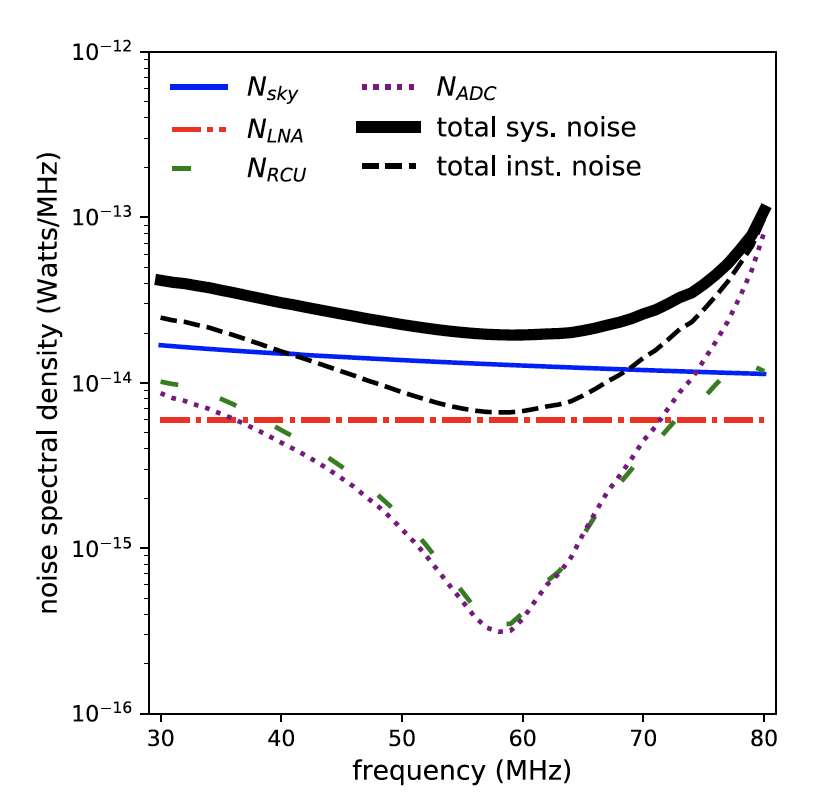
\includegraphics[width=0.44\textwidth]{Figs/LOFAR-antennaNoise,Katie2023-01-30} }
\centering{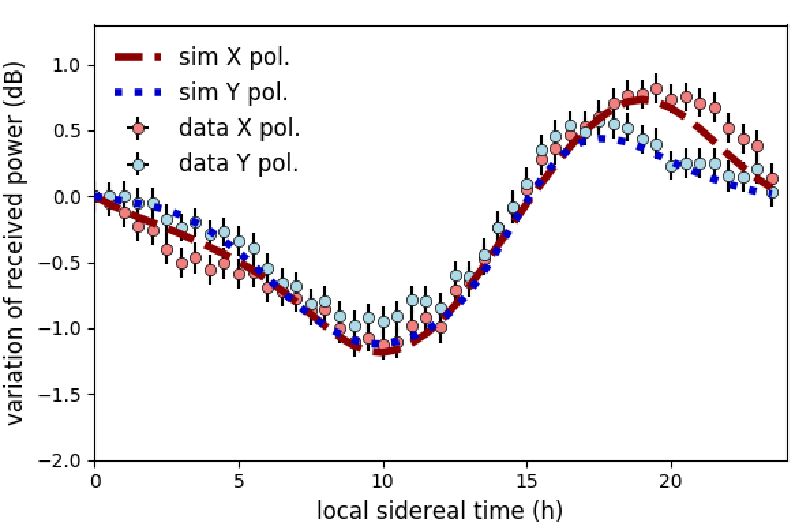
\includegraphics[width=0.54\textwidth]{Figs/KatieFig4Right} }
%\centering{\includegraphics[ bb=1.0cm 2.4cm 24.5cm 25.7cm,clip, width=0.49\textwidth]{../Figs/SE20A7-NPMx_1HIntfSpecSel} }
	\caption{Left: contribution to the noise level for a LOFAR LBA antenna where the antenna-gain has been unfolded. Right: variation of background with siderial time (1~dB=factor 1.26, 3~dB=factor 2, 10~dB=factor 10). Figures 5 and 4-right (Katie Mulrey, January 30, 2023) from \cite{Mulrey:2019}.}	 \figlab{Katie-Fig}
\end{figure}

\figref{Katie-Fig} shows the different contributions to the noise level after unfolding the antenna gain where the galactic noise is integrated over angle folding in the angle dependent antenna gain (normalized to zenith angle). This shows that the number for the total noise level should rather be $P_{n,K}=2.2\times 10^{-14}$~W/MHz when averaged over 30 -- 80~MHz. Note that in averaging over this frequency interval a frequency-weighting, proportional to the antenna gain, should be taken into account.

A source with intensity $St_I$~gb over a slice of duration $\Delta_t$ thus emits a total energy/MHz of
\\$F=0.5\times 4\pi D^2 \times St_I \frac{1\times 10^3}{D^2}\times 1.24\times 10^{-14}\times\frac{\Delta_t}{100ns}\times 10^{-7}$~J/MHz
\\where the first factor $0.5\times 4\pi$ is due to the integration of the dipole intensity over solid angle. Since the electric field is proportional to sinus and the power the square of the E field, this should have been $$\int \sin^2(\theta) d[\cos(\theta)] d\phi=2\pi \int_{-1}^{+1} (1-x^2)\,dx=4\pi(1-1/3)=8\pi/3$$, i.e.\ an extra factor $4/3$ that is not yet included in the following. Reducing this gives
\\$F=2\pi  \times St_I  \times 1.24\times 10^{-18}\times\frac{\Delta_t}{100ns} $~J/MHz


 This yields
$F_O=0.88 \times St_I\times\frac{\Delta_t}{100ns} \times 10^{-17} $~J/MHz $\approx St_I\times\frac{\Delta_t}{100ns} \times 10^{-5} $~pJ/MHz since pico$=10^{-12}$. An additional factor $10^6$ needs to be added because the effective area of the antenna is 1~m$^2$ and not 1~km$^2$

Using Katie's number for the background, \figref{Katie-Fig}, we get $F_K=0.88 (2.2/1.24) \times St_I \times \frac{\Delta_t}{100ns} \times 10^{-17} $~J/MHz $\approx 1.8 \times St_I \times \frac{\Delta_t}{100ns} \times 10^{-5} $~pJ/MHz

The background intensity for a tesseract depends on the distance to the core (increases with the square of the distance) and the number of antennas. The latter is difficult to quantify as this will depend on the intensity they receive as compared to the core, but roughly proportional to their number. The intensity of the brightest background source will increase with the number of voxels in the image cube and should decrease (slightly) with the duration of a slice. For a tesseract at $D^2=2\times 10^3$~km$^2$ and slice of $\Delta_t=100$~ns vertically above the core we obtain for the background noise level $I^n \approx 0.2$~gb. However, the sum of the two transverse components give only $I_{\perp}^n \approx 0.01$~gb. It is seen that for these distances the transverse scales with distance as expected, but the longitudinal intensity tends to diverge for large distances.

The Earth rotation angle (ERA), kind of the same as siderial time, measured in radians, is related to UT1 by a simple linear relation:[3]
\beq  \theta (t_{U})=2\pi (0.779\,057\,273\,2640+1.002\,737\,811\,911\,354\,48\cdot t_{U})
\eeq
where $t_U$ is the Julian UT1 date (JD) minus 2451545.0, that is, 12:00 (midday) Terrestrial Time of January 1, 2000, Unix Timestamp = 946728000. (Note that this differed from 12h UTC on that day by around a minute.)
Katie:  UTC=946728000 gives an LST=19.2 i.e. LST = ERA-.779+.2 = ERA-.58
} % end Omit

\subsubsection{Background}\seclab{SimBckgr}

A dirty guestimate of the background intensity is obtained from the brightness temperature of radiation is given by $T_b = (\lambda^2 / 2k)^{-1} I_\nu$.
Using  ``The Spectrum of the Radio Background Between 13 and 404 MHz'',
A.H.\ Bridle, J.E.\ Baldwin:%https://doi.org/10.1093/mnras/136.2.219
\\Ref~\cite{Bridle:1967}, Fig 10 gives: Brightness $ @60MHz=2.7\times 10^{-21}$~W/m$^2$/Hz/Sr (radiation coming from the North pole).
\\Integrate over the sky as seen by LOFAR (calculation gives Sr=2.3) this gives the energy flux for a LOFAR antenna ($A=1 m^2$ and at 60~MHz) $P_{gb,O}=2.7*2.3\times 10^{-21}$~W/Hz$=6.2\times 10^{-21}$~W/Hz.
\\Assuming the instrumental noise is about the same as the galactic background gives $P_{n,O}=1.24\times 10^{-14}$~W/MHz, however, most of the intensity in $P_{gb}$ comes from the Galactic disk at the equator and the North pole is somewhere in the halo. The mean is thus larger than the value at the North pole which is why Katie's numbers for $P_{gb,K}=1.3\times 10^{-14}$~W/MHz, obtained from an honest integration over sky angle \figref{Katie-Fig}, are larger than Olaf's value $P_{gb,O}=6.2\times 10^{-15}$~W/MHz. Note that $P_{gb,K}$ should depend on siderial time, see~\cite{Mulrey:2019}.


\begin{figure}[th]
\centering{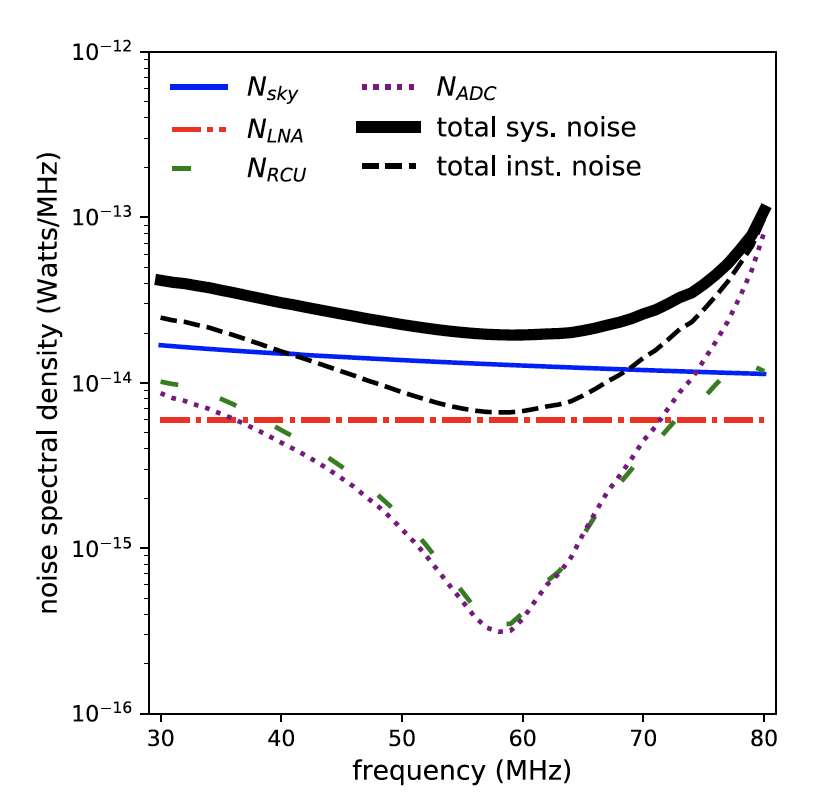
\includegraphics[width=0.44\textwidth]{Figs/LOFAR-antennaNoise,Katie2023-01-30} }
\centering{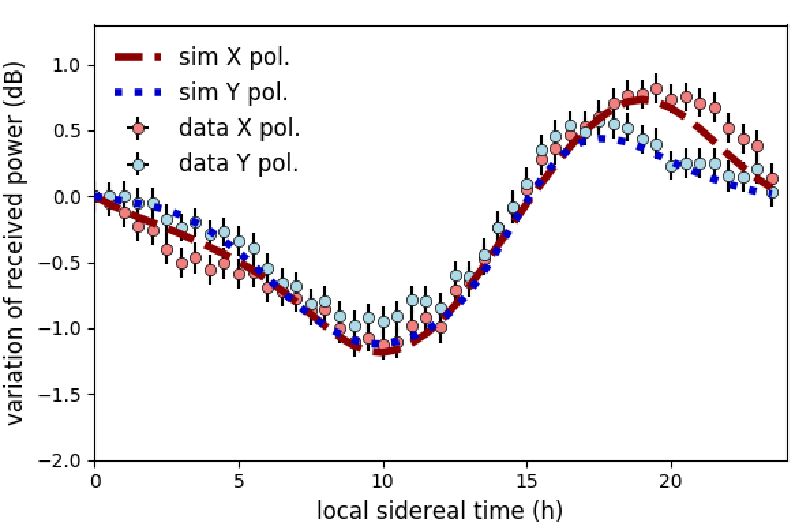
\includegraphics[width=0.54\textwidth]{Figs/KatieFig4Right} }
%\centering{\includegraphics[ bb=1.0cm 2.4cm 24.5cm 25.7cm,clip, width=0.49\textwidth]{../Figs/SE20A7-NPMx_1HIntfSpecSel} }
	\caption{Left: contribution to the noise level for a LOFAR LBA antenna where the antenna-gain has been unfolded. Right: variation of background with siderial time (1~dB=factor 1.26, 3~dB=factor 2, 10~dB=factor 10). Figures 5 and 4-right (Katie Mulrey, January 30, 2023) from \cite{Mulrey:2019}.}	 \figlab{Katie-Fig}
\end{figure}

More accurately \figref{Katie-Fig} shows the different contributions to the noise level after unfolding the antenna gain where the galactic noise is integrated over angle folding in the angle dependent antenna gain (normalized to zenith angle). This shows that the number for the total noise level should rather be $P_{n,K}=2.2\times 10^{-14}$~W/MHz when averaged over 30 -- 80~MHz. Note that in averaging over this frequency interval a frequency-weighting, proportional to the antenna gain, should be taken into account.


The Earth rotation angle (ERA), kind of the same as siderial time, measured in radians, is related to UT1 by a simple linear relation:[3]
\beq  \theta (t_{U})=2\pi (0.779\,057\,273\,2640+1.002\,737\,811\,911\,354\,48\cdot t_{U})
\eeq
where $t_U$ is the Julian UT1 date (JD) minus 2451545.0, that is, 12:00 (midday) Terrestrial Time of January 1, 2000, Unix Timestamp = 946728000. (Note that this differed from 12h UTC on that day by around a minute.)
Katie:  UTC=946728000 gives an LST=19.2 i.e. LST = ERA-.779+.2 = ERA-.58

